\begin{figure}[t]
    \centering
    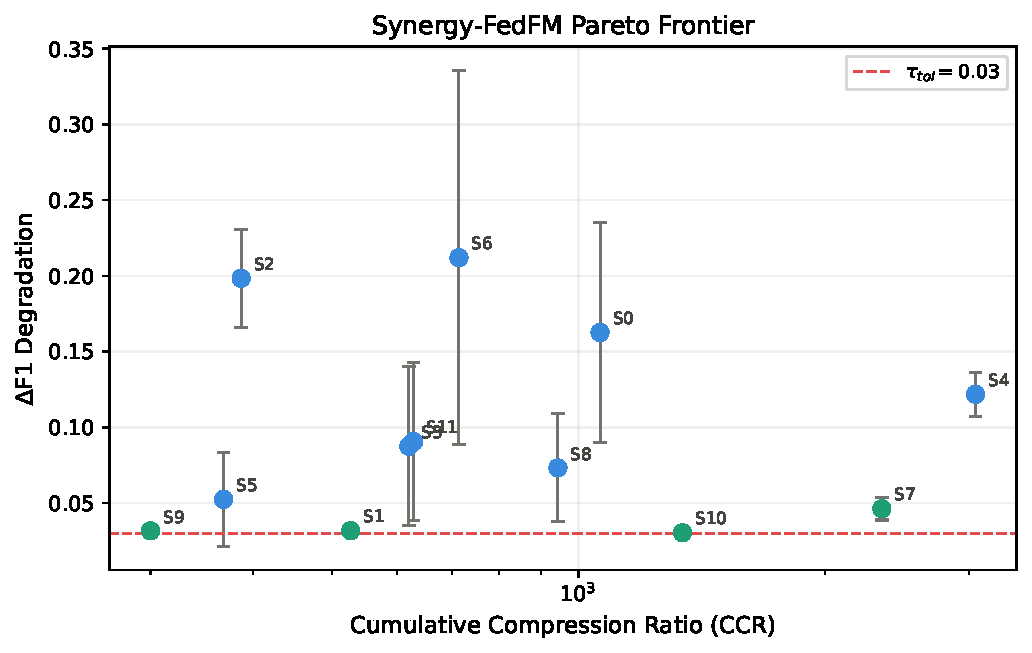
\includegraphics[width=0.92\linewidth]{figures/lhs_pareto_pub.pdf}
    \caption{
        Pareto frontier of the Synergy-FedFM framework across 12 Latin 
        Hypercube Sampling configurations (3 independent seeds each). 
        The x-axis shows the Cumulative Compression Ratio (CCR, log scale) 
        and the y-axis shows F1-score degradation relative to the centralised 
        oracle baseline ($F1_\text{Oracle} = 0.926$). Error bars denote one 
        standard deviation across seeds. The dashed red line marks the 
        operational tolerance bound $\tau_{tol} = 0.03$. Sample S10 
        ($\text{CCR}=1340\times$, $\Delta F1 = 0.030$) represents the optimal 
        configuration $\Phi^*$ satisfying the security constraint while 
        maximising compression. Sample S7 ($\text{CCR}=2348\times$, 
        $\Delta F1 = 0.046$) identifies the empirical breakdown point of 
        the Triple Wall under extreme compression.
    }
    \label{fig:pareto_frontier}
\end{figure}
